\chapter{Fisiologi Tumbuhan Molekuler dan Tanggapan Tekanan}\label{ch:b3:plant-molecular-physiology}

Sebuah semai kacang yang ditumbuhkan di dalam lemari gelap adalah benda yang pucat dan
jangkung: sebuah batang putih panjang, sebuah kait di puncaknya, dua daun kuning yang terlipat. Pindahkanlah
ia ke sebuah jendela dan dalam sehari ia berhenti memanjang, meluruskan
kaitnya, lalu membentangkan dan menghijaukan daunnya --- sebuah jasad yang berbeda, dari
gen yang sama. Ia bukan sedang menunggu tenaga; ia sedang menunggu
keterangan. Sebuah foton merah yang diserap sebuah protein tunggal memberitahunya
bahwa ia telah mencapai cahayanya; nisbah merah terhadap merah-jauh memberitahunya
apakah daun seorang tetangga ada di atasnya; panjang malamnya memberitahunya
musimnya; sebuah penurunan potensial air akarnya, sebuah sentuhan
angin, flagelin sebuah bakteri pada daunnya --- masing-masing dideteksi sebuah
reseptor, diubah menjadi sebuah isyarat kimia, lalu dijawab dengan sebuah perubahan pada
gen mana yang diungkapkan dan sel mana yang tumbuh. Sebuah tumbuhan tidak dapat lari
dari lingkungannya; ia harus membacanya lalu membentuk ulang dirinya. Bab ini
tentang pembacaan itu: fotoreseptornya, \omterm{def:b3:endocrinology:hormone}{hormonnya} dan bagaimana keduanya
bekerja pada skala molekul, tanggapannya terhadap kekeringan, garam, dingin, dan
panas, serta sistem imun dua lapis yang dievolusikan tumbuhan tanpa
satu pun sel yang dapat berpindah.

\section{Membaca cahayanya}

\begin{definition}[Fotoreseptor]\label{def:b3:plant-molecular-physiology:photoreceptors}
\index{fitokrom}\index{kriptokrom}\index{fototropin}%
\index{fotomorfogenesis}\index{etiolasi}
Tumbuhan mengindera cahaya dengan tiga keluarga protein, tidak satu pun berupa
klorofil. \emph{Fitokrom} adalah dimer berpigmen bilin yang
disakelar cahaya merah (\qty{660}{nm}) dari bentuk \emph{Pr} yang tak aktif
ke bentuk \emph{Pfr} yang aktif, lalu kembali oleh merah-jauh (\qty{730}{nm}); Pfr
berpindah ke dalam intinya lalu menandai sebuah keluarga faktor transkripsi, yakni
PIF, untuk dirombak, yang melepaskan gen perkembangan yang tumbuh di cahaya;
di dalam gelap Pfr berbalik perlahan. \emph{Kriptokrom} (biru,
\qty{450}{nm}) adalah flavoprotein yang berkerabat dengan enzim perbaikan DNA,
yang mengendalikan pengurangan etiolasi, jamnya, dan pembungaannya; \emph{fototropin}
(biru) adalah kinase selaput yang mengarahkan pembengkokan ke arah cahaya, yakni
membukanya stomata dan gerakan kloroplas. Sebuah semai di dalam
gelap \emph{teretiolasi} --- hipokotil panjang, kotiledon tertutup, tanpa
klorofil, dengan segenap sumber dayanya dibelanjakan untuk mencapai permukaannya; cahaya
menyakelarnya ke \emph{fotomorfogenesis}, dan sakelarnya dilempar oleh
Pfr dan kriptokrom yang menonaktifkan sebuah kompleks penekan tunggal (COP1)
yang di dalam gelap memusnahkan faktor transkripsi acara cahayanya. Cahaya
dengan demikian dibaca dua kali: sebagai tenaga, oleh kloroplasnya, dan
sebagai isyarat, oleh reseptor yang peka pada fluks foton sejuta kali
lebih kecil.
\end{definition}

\begin{proposition}[Kesetimbangan foto fitokrom]\label{prop:b3:plant-molecular-physiology:photoequilibrium}
\index{kesetimbangan foto}\index{nisbah merah:merah-jauh}\index{penghindaran naungan}
Di bawah cahaya sinambung, Pr dan Pfr saling berubah sampai kedua
laju perubahan fotonya seimbang: dengan $k_{1}$ laju Pr $\to$ Pfr
(yang sebanding dengan fluks merahnya) dan $k_{2}$ laju Pfr $\to$ Pr
(yang sebanding dengan fluks merah-jauhnya, ditambah sedikit dari merahnya, yang juga
diserap Pfr), pecahan bentuk yang aktif adalah
\[
\varphi = \frac{[\text{Pfr}]}{[\text{Pfr}] + [\text{Pr}]} = \frac{k_{1}}{k_{1} + k_{2}},
\]
yang tak bergantung pada fluks totalnya dan ditetapkan hanya oleh \emph{\omterm{prop:b3:plant-molecular-physiology:photoequilibrium}{nisbah
merah:merah-jauh}} $\zeta$ cahayanya. Merah murni memberi $\varphi \approx 0.87$ (Pfr
menyerap sedikit merah pula), merah-jauh murni $0.03$; cahaya siang terbuka, $\zeta \approx
1.15$, memberi sekitar $0.55$, dan cahaya di bawah sebuah kanopi daun, yang
klorofilnya telah mengambil merahnya lalu melewatkan merah-jauhnya, punya
$\zeta \approx 0.2$ dan $\varphi \approx 0.2$. Sebuah tumbuhan membaca
$\varphi$-nya sebagai kehadiran tetangga: sebuah nilai yang rendah memicu
sindrom \emph{\omterm{prop:b3:plant-molecular-physiology:photoequilibrium}{penghindaran naungan}} --- batang yang memanjang, daun yang terangkat,
pembungaan yang dini, percabangan yang lebih sedikit --- lewat PIF yang tidak lagi
dimusnahkan Pfr. Penanaman rapat seorang petani adalah sebuah lomba penghindar naungan;
gandum kerdil Revolusi Hijau, yang tak peka pada isyarat itu, menaruh
pertumbuhan yang dihematnya ke dalam bulirnya.
\end{proposition}
\begin{proof}
$\mathrm{d}[\text{Pfr}]/\mathrm{d}t = k_{1}[\text{Pr}] - k_{2}[\text{Pfr}]$
dengan $[\text{Pr}] + [\text{Pfr}] = P$ yang terpancang memberi, pada keadaan mantap,
$k_{1}(P - [\text{Pfr}]) = k_{2}[\text{Pfr}]$, yang darinya $\varphi = k_{1}/
(k_{1} + k_{2})$. Kedua lajunya sebanding dengan fluks yang datang, sehingga
menskalakan cahayanya menskalakan keduanya lalu membiarkan $\varphi$ tak berubah; hanya
susunan spektrumnya yang berarti. Keadaan mantapnya didekati dengan laju
$k_{1} + k_{2}$ --- hitungan detik di bawah sinar matahari, hitungan menit pada senja --- dan
pembalikan gelap Pfr, dengan paruh hidup berjam-jam, menetapkan apa yang tersisa pada
malam hari.
\end{proof}

\begin{omfigure}
\begin{tikzpicture}[every node/.style={font=\scriptsize}, >=stealth]
  \node[draw, very thick, omDef, fill=omDef!15, rounded corners, minimum width=1.6cm, minimum height=0.9cm] (pr) at (0,0) {Pr (tak aktif)};
  \node[draw, very thick, omThm, fill=omThm!15, rounded corners, minimum width=1.6cm, minimum height=0.9cm] (pfr) at (4.2,0) {Pfr (aktif)};
  \draw[->, very thick, red!70!black] (pr.north east) to[bend left=25] node[above] {merah, \qty{660}{nm}} (pfr.north west);
  \draw[->, very thick, red!40!black] (pfr.south west) to[bend left=25] node[below] {merah-jauh, \qty{730}{nm}} (pr.south east);
  \draw[->, thick, gray] (pfr.south) ++(0.5,-0.15) to[bend left=40] node[right, font=\tiny, gray] {pembalikan gelap, berjam-jam} ++(-0.3,-0.9);
  \draw[->, thick] (pfr.east) -- ++(1.0,0) node[right, align=left] {ke dalam intinya:\\PIF dirombak, COP1 mati;\\acara tumbuh-cahaya menyala};
  \begin{scope}[shift={(0,-4.6)}]
  \begin{axis}[
    width=0.55\linewidth, height=4.6cm,
    axis x line=bottom, axis y line=left,
    xmin=0, xmax=2.5, ymin=0, ymax=1,
    xlabel={nisbah merah:merah-jauh $\zeta$}, ylabel={$\varphi = $ pecahan Pfr},
    xlabel style={font=\scriptsize, at={(axis description cs:0.5,-0.15)}, anchor=north}, ylabel style={font=\scriptsize},
    tick label style={font=\scriptsize}, xtick={0.2,0.5,1.15,2}, xticklabels={0.2,0.5,1.15,2}, ytick={0.2,0.55,0.87},
    clip=false,
  ]
  \addplot[very thick, omDef, domain=0:2.5, samples=80] {0.87*x/(x+0.6)};
  \draw[dashed, gray] (axis cs:0.2,0) -- (axis cs:0.2,0.22) -- (axis cs:0,0.22);
  \draw[dashed, gray] (axis cs:1.15,0) -- (axis cs:1.15,0.57) -- (axis cs:0,0.57);
  \node[font=\tiny, anchor=west, align=left] at (axis cs:0.25,0.12) {di bawah sebuah kanopi:\\penghindaran naungan};
  \node[font=\tiny, anchor=south west] at (axis cs:1.2,0.62) {cahaya siang terbuka};
  \node[font=\tiny, anchor=north west, omDef, align=left] at (axis cs:1.6,0.45) {sebuah cocokan empiris,\\$\varphi \approx 0.87\,\zeta/(\zeta + 0.6)$};
  \end{axis}
  \end{scope}
\end{tikzpicture}

{\small Sakelar \omterm{def:b3:plant-molecular-physiology:photoreceptors}{fitokromnya}. Cahaya merah membuat bentuk yang aktif,
merah-jauh membatalkannya, kegelapan perlahan membalikkannya; pecahan mantap bentuk
yang aktif bergantung pada imbangan warna cahayanya dan bukan pada
kecerahannya, dan begitulah sebuah semai tahu sebuah daun ada di atasnya.}
\end{omfigure}

\begin{proof}[Bukti eksperimental]
Borthwick, Hendricks, dan rekannya (1952) memberi biji selada kilatan
singkat: merah membuatnya berkecambah, merah-jauh yang diberikan sesudahnya membatalkannya,
merah lagi memulihkannya, dan seterusnya sepanjang selusin pergantian --- kilatan
terakhirlah yang memutuskan, yakni tanda tangan sebuah pigmen yang terbalikkan, yang lalu
mereka petik (1959) sebagai sebuah protein biru yang mengubah spektrum
serapannya di bawah merah dan merah-jauh. Seluruh acara semai yang
tumbuh dalam gelap kemudian terbukti bergantung pada satu penekan: mutan tanpa
COP1 berkembang dalam gelap total seolah-olah dalam cahaya, pendek dan siap menghijau,
dan mutan yang kekurangan \omterm{def:b3:plant-molecular-physiology:photoreceptors}{fitokrom} serta \omterm{def:b3:plant-molecular-physiology:photoreceptors}{kriptokrom} tetap teretiolasi di dalam
cahaya.
\end{proof}

\begin{omfigure}
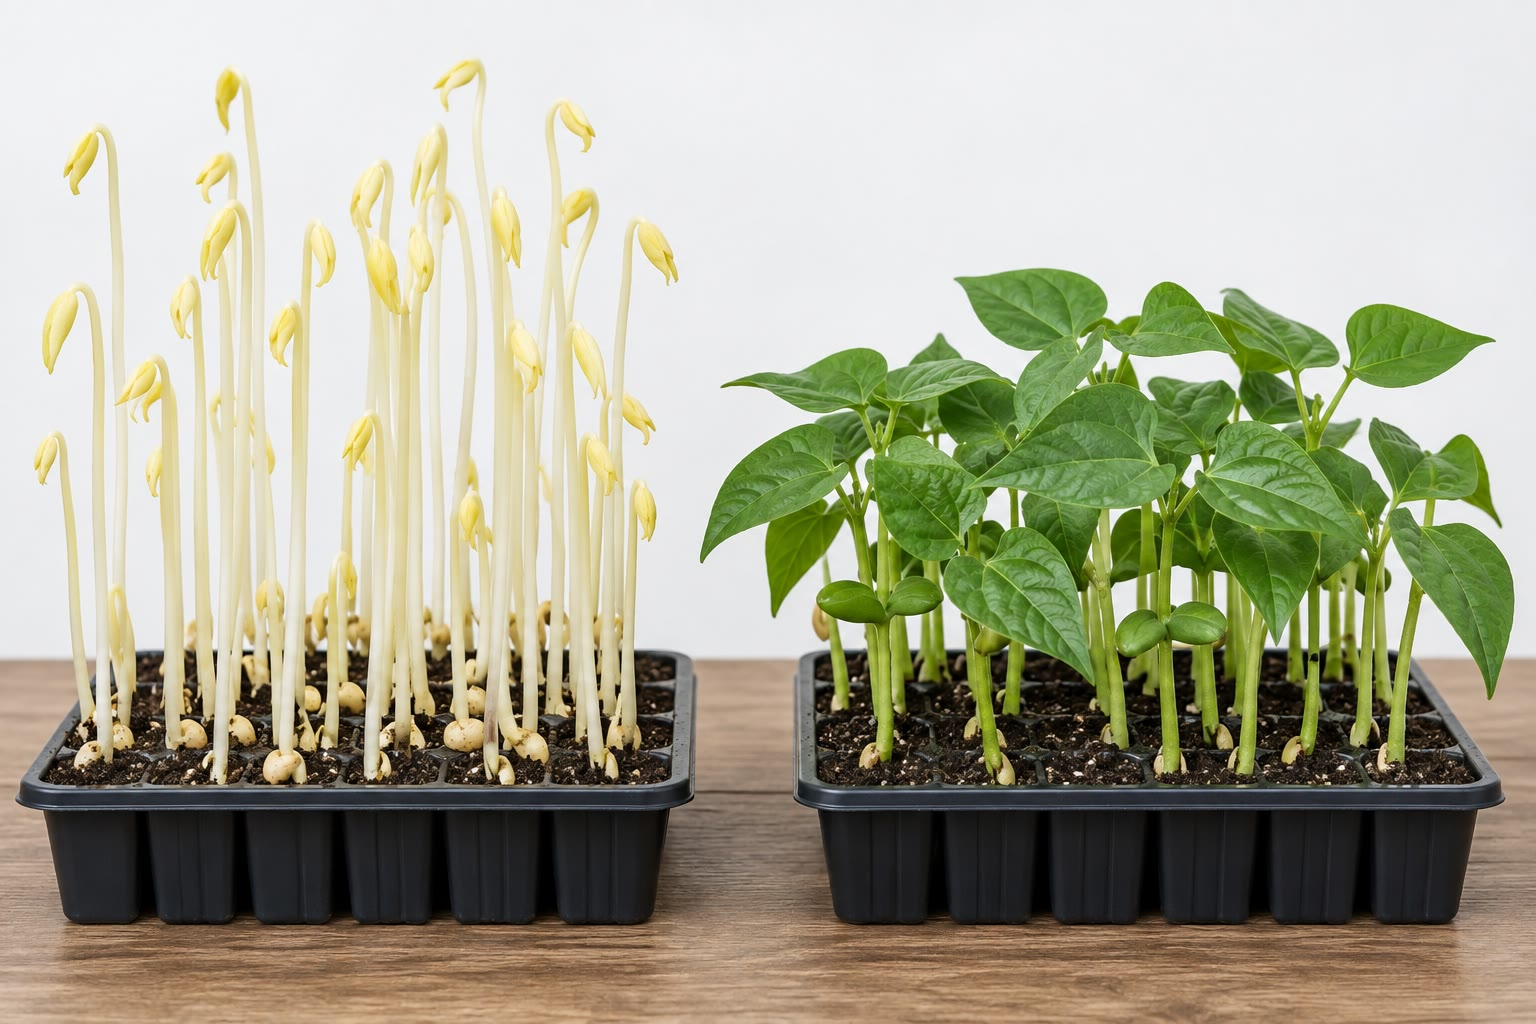
\includegraphics[width=0.56\linewidth]{images/book5/ai/b5-22-etiolated-seedlings.jpg}

{\small Semai yang ditumbuhkan dalam gelap dan dalam cahaya: genom yang sama,
dua acara perkembangan, dan perbedaannya adalah sebuah foton merah tunggal
yang diserap \omterm{def:b3:plant-molecular-physiology:photoreceptors}{fitokrom}.}
\end{omfigure}

\section{Hormon pada skala molekul}

\begin{definition}[Hormon tumbuhan dan reseptornya]\label{def:b3:plant-molecular-physiology:hormones}
\index{auksin}\index{TIR1}\index{giberelin}\index{DELLA}%
\index{asam absisat}\index{etilena}\index{sitokinin}\index{brasinosteroid}
Jilid Tahun~1 memerikan apa yang dilakukan \omterm{def:b3:endocrinology:hormone}{hormon} tumbuhan; di sini adalah bagaimana
\omterm{def:b3:endocrinology:hormone}{hormon} itu didengar. Beberapa bekerja lewat \emph{pemusnahan yang teratur}.
\emph{Auksin} (asam indol-3-asetat) mengikat protein F-box
\emph{TIR1}, yang merekatkannya pada penekan Aux/IAA, yang lalu
diubikuitinasi dan dimusnahkan proteasomnya: gen tanggapan auksin
yang ditekannya menyala dalam hitungan menit --- \omterm{def:b3:endocrinology:hormone}{hormonnya} adalah sebuah
perekat molekuler, dan reseptornya bagian dari mesin perombakannya.
\emph{Giberelin} melakukan hal yang sama dengan penekan \emph{DELLA} milik
pertumbuhannya, lewat reseptornya GID1: gandum dan padi kerdil
Revolusi Hijau mengusung protein DELLA yang tidak dapat dimusnahkan, sehingga
tetap pendek berapa pun giberelin yang dibuatnya. \emph{Jasmonat}
mengikuti logika yang sama dengan penekan JAZ. \emph{Asam absisat}
(ABA), yakni \omterm{def:b3:endocrinology:hormone}{hormon} kekeringan dan kelelapan, mengikat reseptor PYR/PYL,
yang lalu menghambat sebuah fosfatase (PP2C), yang melepaskan sebuah kinase
(SnRK2) yang memfosforilasi saluran ion dan faktor transkripsi ---
yakni sebuah negatif rangkap yang membuat tanggapannya curam. \emph{Etilena}, sebuah
gas, mengikat reseptor bertembaga di dalam selaput RE yang pada ketiadaannya
secara aktif menekan tanggapannya; pengikatannya mematikannya, lalu
gen pemasakan, penuaan, dan tekanannya menyala. \emph{Sitokinin}
bekerja lewat reseptor histidin-kinase seperti \omterm{def:b3:bacteriology:quorum}{sistem dua komponen}
bakteri; \emph{brasinosteroid}, yakni steroid tumbuhan, lewat
sebuah kinase reseptor di permukaan, bukan sebuah \omterm{def:b3:endocrinology:hormone}{reseptor inti} --- yakni satu-satunya \omterm{def:b3:endocrinology:hormone}{hormon
steroid} di mana pun yang didengar di permukaan sel. Tumbuhan tidak punya kelenjar: tiap
\omterm{def:b3:endocrinology:hormone}{hormonnya} dibuat di tempat ia diperlukan, atau dipindahkan pengusung khas, dan
kepekatannya ditetapkan setempat lewat sintesis, konjugasi, dan
pemusnahan.
\end{definition}

\begin{theorem}[Pengangkutan auksin berkutub secara kemiosmosis]\label{thm:b3:plant-molecular-physiology:auxin}
\index{pengangkutan auksin berkutub}\index{protein PIN}\index{penjebakan anion}
Asam indol-3-asetat adalah sebuah asam lemah, $\mathrm{p}K_{a} = 4.75$. Di dalam
ruang dinding selnya pada pH~$5.5$, sebuah pecahan yang berarti berupa IAAH yang
netral, yang membaur melintasi selaputnya; di dalam sitosolnya pada pH~$7.2$
nyaris semuanya berupa anion IAA$^{-}$, yang tidak dapat pergi lewat pembauran. Pada
kesetimbangan bentuk netralnya melintasi selaputnya, nisbah total
\omterm{def:b3:plant-molecular-physiology:hormones}{auksin} di dalam terhadap di luar adalah
\[
\frac{[\text{IAA}]_{\text{dalam}}}{[\text{IAA}]_{\text{luar}}}
= \frac{1 + 10^{\,\mathrm{pH}_{\text{dalam}} - \mathrm{p}K_{a}}}{1 + 10^{\,\mathrm{pH}_{\text{luar}} - \mathrm{p}K_{a}}}
\approx \frac{283}{6.6} \approx 43 :
\]
selnya menjebak \omterm{def:b3:plant-molecular-physiology:hormones}{auksinnya} empat puluh kali lipat. \omterm{def:b3:plant-molecular-physiology:hormones}{Auksinnya} hanya dapat pergi lewat
pengusung keluar \emph{PIN}, dan karena tiap selnya menaruh PIN-nya pada satu
muka --- muka basal pada batangnya --- \omterm{def:b3:plant-molecular-physiology:hormones}{auksin} yang diambil dari segala arah
pergi di bagian bawahnya, memasuki sel berikutnya, dan seterusnya: sebuah kolom
sel dengan kekutuban yang sama adalah sebuah ban berjalan yang memindahkan \omterm{def:b3:plant-molecular-physiology:hormones}{auksin} pada sekitar
\qty{1}{cm/h} dari pucuk tunas ke akarnya, dan mengarahkan ulang PIN-nya
mengarahkan ulang alirannya, dan begitulah sisi batang yang ternaungi berakhir
memuat lebih banyak \omterm{def:b3:plant-molecular-physiology:hormones}{auksin} lalu tumbuh lebih cepat.
\end{theorem}
\begin{proof}
Henderson--Hasselbalch: $[\text{IAA}^{-}]/[\text{IAAH}] = 10^{\,\mathrm{pH}
- \mathrm{p}K_{a}}$, sehingga totalnya $= [\text{IAAH}](1 + 10^{\,\mathrm{pH} -
\mathrm{p}K_{a}})$. Bentuk netralnya menyeimbang, $[\text{IAAH}]_{\text{dalam}}
= [\text{IAAH}]_{\text{luar}}$; membagi totalnya memberi nisbahnya,
$(1 + 10^{2.45})/(1 + 10^{0.75}) = 283/6.6$. Dengan PIN pada satu muka,
satu-satunya jalan keluar anionnya berarah; sebuah kolom berisi $n$ sel meneruskan
fluksnya, dan laju yang terukur, seorde lebih besar daripada
pembauran pada jarak ini, adalah laju keluaran yang diperantarai pengusung pada
tiap batas selnya. Hipotesis Cholodny--Went (dasawarsa 1920-an) bahwa pembengkokannya
mengikuti sebuah pengagihan ulang \omterm{def:b3:plant-molecular-physiology:hormones}{auksin} ke samping dibenarkan lewat
pengukuran langsung pada koleoptil oat dan lewat pencitraan perpindahan PIN pada
akar \emph{Arabidopsis} yang dibaringkan pada sisinya (dasawarsa 2000-an).
\end{proof}

\begin{omfigure}
\begin{tikzpicture}[every node/.style={font=\scriptsize}, >=stealth]
  % three cells in a column
  \foreach \y in {0,-2.2,-4.4} {
    \draw[thick, omDef, fill=omDef!8] (0,\y) rectangle (3.2,\y-1.9);
    \draw[very thick, omThm] (0.6,\y-1.9) -- (2.6,\y-1.9);
    \node[right, font=\tiny] at (3.3,\y-0.4) {sitosol pH 7.2};
    \node[right, font=\tiny] at (3.3,\y-0.8) {IAA$^{-}$ terjebak};
    \draw[->, thick, omDef!70!black] (-0.6,\y-0.6) -- (0.4,\y-0.6); \node[left, font=\tiny] at (-0.6,\y-0.6) {IAAH masuk};
    \draw[->, thick, omDef!70!black] (3.8,\y-1.3) -- (2.8,\y-1.3);
    \draw[->, very thick, omThm] (1.6,\y-1.5) -- (1.6,\y-2.35);
  }
  \node[left, align=right, font=\tiny] at (-0.6,-1.4) {dinding pH 5.5:\\\qty{15}{\%} IAAH,\\\qty{85}{\%} IAA$^{-}$};
  \node[omThm, right, font=\tiny] at (3.3,-2.05) {pengusung keluar PIN, muka basal saja};
  \node[above] at (1.6,0.1) {pucuk tunas: sumber auksin};
  \node[below] at (1.6,-6.8) {ke arah akarnya, \qty{1}{cm/h}};
  \node[right, align=left] at (5.4,-3.6) {dalam : luar $\approx 43 : 1$\\(penjebakan anionnya)\\[3pt]keluar hanya lewat PIN,\\sehingga kolomnya sebuah ban berjalan;\\pindahkanlah PIN-nya ke sebuah muka samping\\dan alirannya berbelok};
\end{tikzpicture}

{\small Model kemiosmosis \omterm{thm:b3:plant-molecular-physiology:auxin}{pengangkutan auksin berkutub}. Asamnya masuk lewat
muka mana pun sebagai molekul netralnya, terjebak sebagai anion pada pH
sitosolnya, lalu pergi hanya lewat pengusung yang telah ditaruh selnya pada
satu muka --- sehingga sederet sel meneruskan \omterm{def:b3:plant-molecular-physiology:hormones}{auksinnya} ke satu arah.}
\end{omfigure}

\begin{example}[Gravitropisme dan fototropisme]\label{ex:b3:plant-molecular-physiology:tropism}
Baringkanlah sebuah semai pada sisinya. Di dalam tudung akarnya, plastid padat berisi
pati mengendap ke sisi bawah yang baru pada sel kolumelanya dalam hitungan
menit; pengusung PIN3 sel itu berpindah ke muka bawahnya;
\omterm{def:b3:plant-molecular-physiology:hormones}{auksinnya} mengalir lebih banyak menuruni sayap bawah akarnya, tempat ia, karena
di atas optimum bagi sel akarnya, \emph{menghambat} pemanjangan, lalu
akarnya melengkung ke bawah. Pada tunasnya, aliran ke samping yang sama ke sisi
bawahnya justru \emph{mendorong} pemanjangan (optimum sel tunasnya lebih tinggi),
lalu tunasnya melengkung ke atas. Fototropisme: \omterm{def:b3:plant-molecular-physiology:photoreceptors}{fototropin} pada sisi yang tersinari
sebuah tunas mengubah penaruhan PIN sehingga \omterm{def:b3:plant-molecular-physiology:hormones}{auksinnya} menimbun pada sisi yang
ternaungi, yang tumbuh lebih cepat, lalu membengkokkan tunasnya ke arah cahayanya. Kedua
gerakannya lambat --- berjam-jam --- sebab keduanya pertumbuhan, bukan gerak,
dan keduanya tak terpulihkan pada jaringan yang telah tumbuh. Darwin (1880)
menunjukkan bahwa pucuk sebuah semai rumput menanggapi cahayanya dan daerah
di bawahnya membengkok; Went (1928) mengumpulkan pengaruhnya di dalam sebuah balok agar yang ditaruh
pada sebuah pucuk yang dipotong lalu menunjukkan bahwa sebuah balok yang ditaruh tidak setangkup pada sebuah
tunas yang dipenggal membuatnya membengkok: pengaruhnya berupa sebuah zat yang dapat membaur, yang
lalu dinamai \omterm{def:b3:plant-molecular-physiology:hormones}{auksin}.
\end{example}

\section{Air, garam, dingin, dan panas}

\begin{definition}[Tekanan abiotik]\label{def:b3:plant-molecular-physiology:abiotic}
\index{tekanan kekeringan}\index{penyesuaian osmosis}\index{tekanan garam}%
\index{penyesuaian dingin}\index{protein kejut panas}
Sebuah tumbuhan tidak dapat lolos, sehingga ia mengeraskan diri. \emph{Kekeringan}: potensial air
yang turun di akarnya memicu sintesis ABA; ABA menutup stomatanya dalam
hitungan menit, lalu sepanjang hari menyalakan gen bagi \emph{penyesuaian osmosis}
(prolin, gula, dan zat terlarut serasi lain menimbun, yang menurunkan
potensial air selnya sehingga ia terus menarik air), bagi dehidrin yang
melindungi protein, dan bagi luas daun yang lebih kecil serta akar yang lebih dalam.
\emph{Garam} adalah kekeringan ditambah racun: natriumnya masuk lewat saluran kalium
lalu bersaing dengan kaliumnya; tumbuhan yang tahan memompanya kembali ke luar
akarnya (jalur SOS), ke dalam vakuolanya (penukar NHX), atau mengekskresikannya
dari kelenjar daunnya, dan ujung \emph{halofit}-nya hidup di dalam air laut.
\emph{Dingin}: kedinginan mengakukan selaput lalu memperlambat enzimnya; pembekuan
menarik air dari selnya ke dalam es luar selnya lalu mengeringkannya.
\emph{Penyesuaian dingin} --- sepekan hari yang sejuk --- memicu faktor
transkripsi CBF, yang menyalakan ratusan gen bagi
lipid pencair selaput, gula, protein antibeku, dan dehidrin,
dan sebuah rai musim dingin yang akan mati pada \qty{-5}{\celsius} pada bulan Agustus bertahan
pada \qty{-30}{\celsius} pada bulan Januari. \emph{Panas} membuka \omterm{def:b3:structural-biology:levels}{lipatan} protein; dalam
beberapa menit sesudah sebuah kenaikan, sebuah faktor kejut panas melepaskan \emph{protein kejut
panas}, yakni \omterm{def:b3:structural-biology:chaperones}{pendamping} yang melipat ulang atau membuangnya, dari keluarga yang sama
seperti pada tiap jasad. \emph{Banjir} membuat akarnya kelaparan oksigen;
padi membuat saluran udara (aerenkima) lalu memanjang untuk menjaga daunnya
di atas airnya, dengan \omterm{def:b3:plant-molecular-physiology:hormones}{etilena} menjadi isyarat yang menimbun ketika ia tidak dapat
lolos ke dalam airnya. Banyak acara ini bertindihan --- ABA, spesies oksigen
reaktif, dan lonjakan kalsium adalah pesuruh kedua yang dipakai bersama --- dan sebuah
tumbuhan yang tersesuaikan pada satu tekanan kerap sebagian terlindungi terhadap
tekanan lain.
\end{definition}

\begin{proposition}[Stoma sebagai sebuah katup]\label{prop:b3:plant-molecular-physiology:stomata}
\index{stoma}\index{sel penjaga}%
\index{kehantaran stomata}\index{kemangkusan pemakaian air}
Sepasang \emph{\omterm{prop:b3:plant-molecular-physiology:stomata}{sel penjaga}} membatasi tiap liang stomatanya; liangnya membuka
ketika keduanya mengambil kalium dan anion (lalu membuat gula), mengembang, lalu
melengkung terpisah, dan menutup ketika keduanya kehilangannya. Cahaya biru (\omterm{def:b3:plant-molecular-physiology:photoreceptors}{fototropin}),
CO$_{2}$ rendah, dan kelembapan membukanya; kegelapan, CO$_{2}$ tinggi, kekeringan, dan
ABA menutupnya. Rute ABA: reseptor $\to$ fosfatase terhambat $\to$
kinase aktif $\to$ saluran anion (SLAC1) terbuka $\to$ selaputnya
terdepolarisasi $\to$ kaliumnya pergi lewat saluran keluar $\to$ airnya
mengikuti $\to$ liangnya menutup, dalam sepuluh menit. Liangnya adalah tempat
perdagangan pusat tumbuhannya dilakukan: CO$_{2}$ membaur masuk dan uap air
keluar lewat lubang yang sama, dan karena landaian uapnya (sebuah daun pada
kelembapan \qty{100}{\%} di dalamnya terhadap udara pada \qty{50}{\%}) lima puluh
kali lebih curam daripada landaian CO$_{2}$-nya (\qty{400}{ppm} di luar,
\qty{250}{} di dalam), sehelai daun kehilangan beberapa ratus molekul air
tiap molekul karbon yang difiksasinya. \emph{\omterm{prop:b3:plant-molecular-physiology:stomata}{Kehantaran stomata}}
$g_{s}$ menetapkan kedua fluksnya: transpirasinya $E = g_{s}\,\Delta w$ dan
asimilasinya $A = (g_{s}/1.6)\,\Delta c$ (karena CO$_{2}$ lebih berat, ia
membaur $1.6$ kali lebih lambat), sehingga \emph{\omterm{prop:b3:plant-molecular-physiology:stomata}{kemangkusan pemakaian air}}
$A/E = \Delta c/(1.6\,\Delta w)$ bergantung pada landaiannya, bukan pada seberapa
lebar liangnya terbuka; menutup liangnya menurunkan kedua fluksnya bersama-sama, dan
menaikkan CO$_{2}$ dalamnya (tumbuhan C$_{4}$, yang memekatkannya) atau
membuka hanya pada malam hari (tumbuhan CAM, di dalam udara sejuk yang lembap) adalah cara tumbuhan
gurun memperbaiki nisbahnya.
\end{proposition}
\begin{proof}
Hukum Fick melintasi liangnya bagi tiap gasnya, dengan kehantaran geometris yang sama
yang diskalakan nisbah koefisien pembaurannya
$D_{\mathrm{H_2O}}/D_{\mathrm{CO_2}} = 1.6$; membagi kedua fluksnya
meniadakan $g_{s}$. Angkanya: $\Delta w \approx \qty{15}{mmol/mol}$ udara
pada \qty{25}{\celsius} dan kelembapan \qty{50}{\%}, $\Delta c \approx
\qty{150}{\micro mol/mol}$: $A/E = 150/(1.6\times\num{15000}) = 1/160$
--- yakni $160$ molekul air tiap CO$_{2}$ pada keadaan yang sejuk itu,
$500$ pada udara kering. Urutan kerja ABA digarap dengan
protoplas \omterm{prop:b3:plant-molecular-physiology:stomata}{sel penjaga} di bawah penjepit petak, dengan arus anionnya muncul
dalam semenit sesudah ABA dan mutan tanpa SLAC1 gagal menutup.
\end{proof}

\begin{omfigure}
\begin{tikzpicture}[every node/.style={font=\scriptsize}, >=stealth]
  % pore with two guard cells
  \begin{scope}[shift={(0,0)}]
    \fill[omProp!30] (0,0) ellipse (1.4 and 0.9);
    \fill[white] (0,0) ellipse (0.5 and 0.6);
    \draw[thick, omProp!80!black] (0,0) ellipse (1.4 and 0.9); \draw[thick, omProp!80!black] (0,0) ellipse (0.5 and 0.6);
    \node[below, font=\tiny] at (0,-1.0) {terbuka: K$^{+}$, Cl$^{-}$, malat masuk, tegang};
    \draw[->, thick, omDef] (0,0.3) -- (0,1.5) node[above, font=\tiny] {H$_2$O keluar, $E = g_{s}\Delta w$};
    \draw[->, thick, omThm] (0,1.5) ++(-1.0,0) -- ++(0,-1.2); \node[left, font=\tiny, omThm] at (-1.1,1.0) {CO$_2$ masuk, $A = g_{s}\Delta c/1.6$};
  \end{scope}
  \begin{scope}[shift={(4.2,0)}]
    \fill[omProp!30] (0,0) ellipse (1.2 and 0.75);
    \draw[thick, omProp!80!black] (0,0) ellipse (1.2 and 0.75); \draw[very thick, omProp!80!black] (0,-0.5) -- (0,0.5);
    \node[below, font=\tiny] at (0,-0.9) {tertutup: ionnya hilang, lembek};
  \end{scope}
  \draw[->, thick] (1.6,0) -- (2.8,0) node[midway, above, font=\tiny] {ABA, gelap,};
  \node[font=\tiny] at (2.2,-0.25) {CO$_2$ tinggi};
  % ABA pathway chain
  \begin{scope}[shift={(7.0,1.7)}]
    \node[draw, rounded corners, fill=omDef!20, align=center, font=\tiny] (a) at (0,0) {ABA mengikat\\PYR/PYL};
    \node[draw, rounded corners, fill=omThm!15, align=center, font=\tiny] (b) at (0,-0.9) {fosfatase PP2C\\terhambat};
    \node[draw, rounded corners, fill=omMeth!25, align=center, font=\tiny] (c) at (0,-1.8) {kinase SnRK2\\aktif};
    \node[draw, rounded corners, fill=omProp!25, align=center, font=\tiny] (d) at (0,-2.7) {saluran anion SLAC1\\terbuka: depolarisasi};
    \node[draw, rounded corners, fill=omProp!25, align=center, font=\tiny] (e) at (0,-3.6) {K$^{+}$ keluar, air keluar,\\liangnya menutup dalam \qty{10}{min}};
    \draw[-|, thick] (a) -- (b); \draw[-|, thick] (b) -- (c); \draw[->, thick] (c) -- (d); \draw[->, thick] (d) -- (e);
    \node[right, font=\tiny, align=left] at (1.5,-0.9) {dua penghambatan\\berderet:\\sebuah sakelar yang curam};
  \end{scope}
\end{tikzpicture}

{\small Stoma dan isyarat yang menutupnya. Air dan karbon dioksida
berbagi liangnya, sehingga tumbuhannya menukar yang satu dengan yang lain pada sebuah laju yang ditetapkan
kedua landaiannya; \omterm{def:b3:endocrinology:hormone}{hormon} kekeringan menutup katupnya lewat sebuah rantai
dua penghambatan, yang membuat tanggapannya serupa sakelar.}
\end{omfigure}

\begin{omfigure}
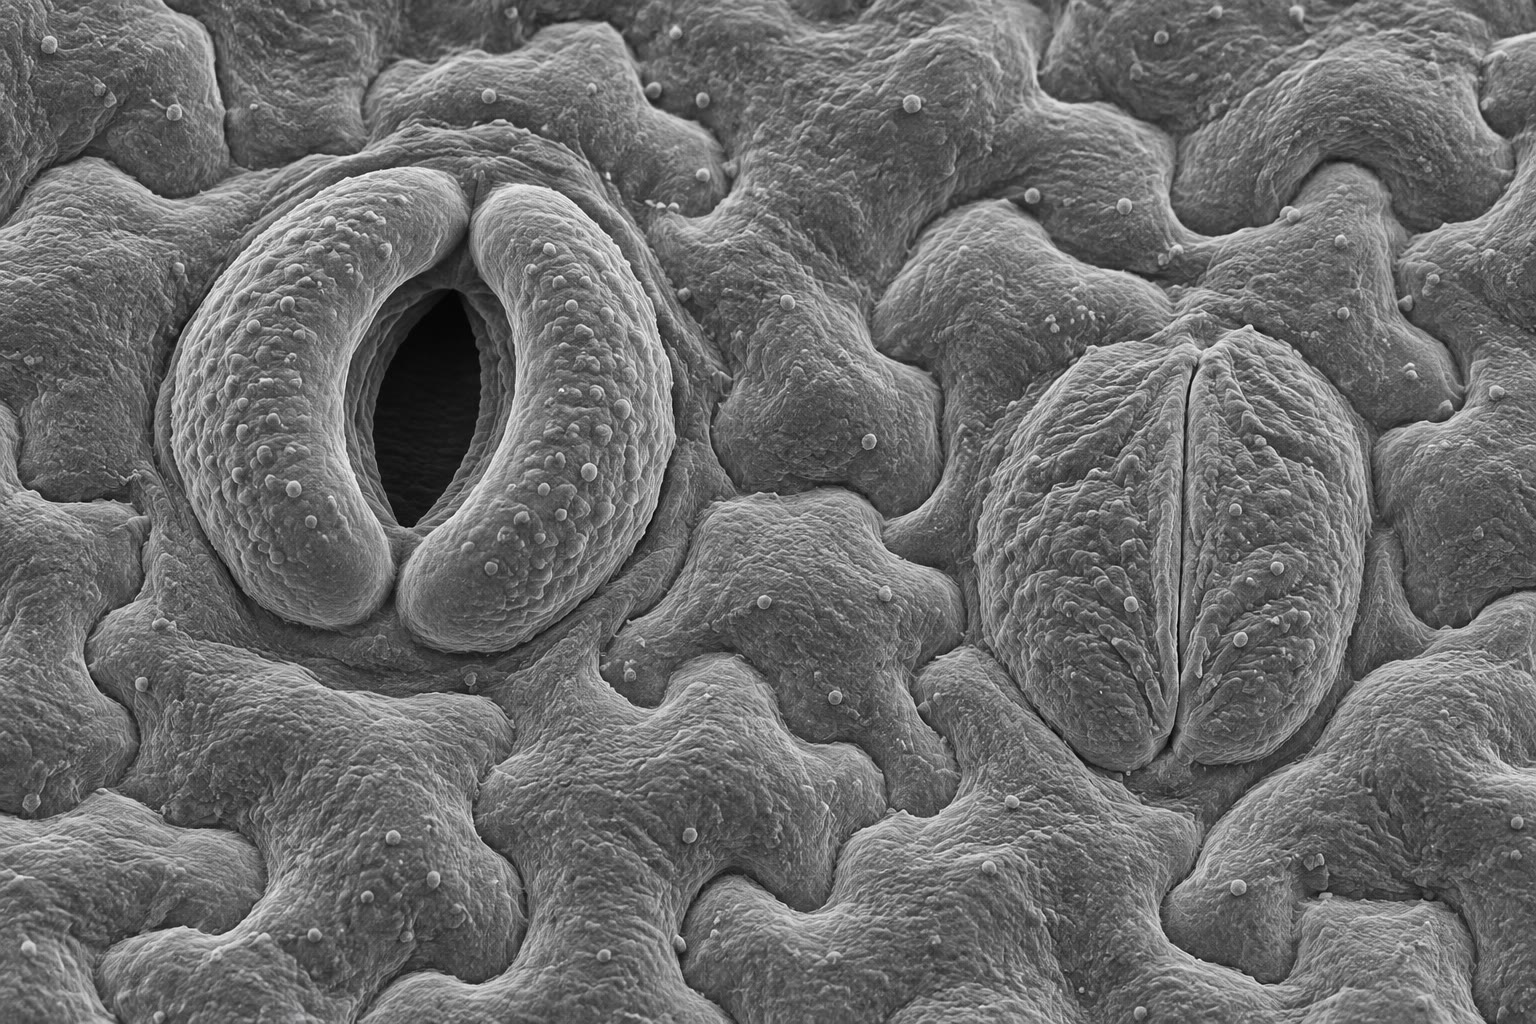
\includegraphics[width=0.46\linewidth]{images/book5/ai/b5-22-stomata-sem.jpg}\hspace{0.04\linewidth}
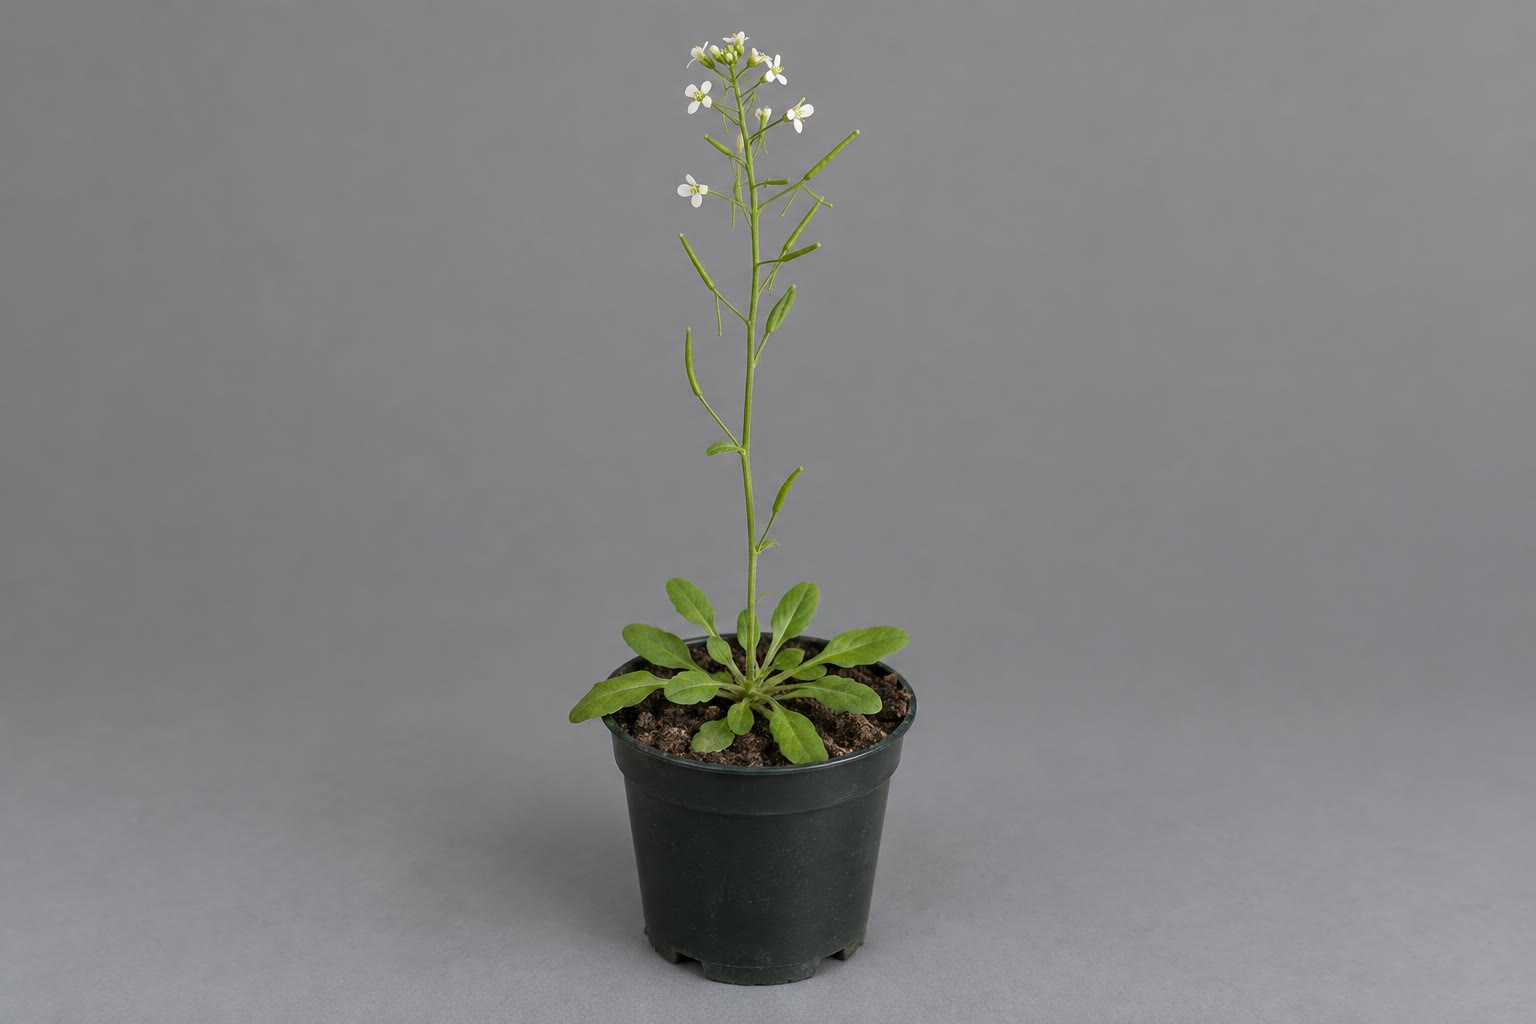
\includegraphics[width=0.46\linewidth]{images/book5/ai/b5-22-arabidopsis.jpg}

{\small Kiri: stomata pada sebuah permukaan daun, tiap liangnya di antara kedua
\omterm{prop:b3:plant-molecular-physiology:stomata}{sel penjaganya}, sebagian terbuka dan sebagian tertutup. Kanan: \emph{Arabidopsis
thaliana}, sebuah gulma pinggir jalan bergenom kecil, berangkatan enam minggu, dan
bergalur mutan seratus ribu, yang di dalamnya kebanyakan molekul bab ini
ditemukan.}
\end{omfigure}

\section{Imunitas tanpa sel imun}

\begin{definition}[Dua lapis imunitas tumbuhan]\label{def:b3:plant-molecular-physiology:immunity}
\index{imunitas terpicu pola}\index{imunitas terpicu efektor}%
\index{reseptor NLR}\index{tanggapan hipersensitif}\index{kekebalan perolehan menyeluruh}%
\index{asam salisilat}\index{asam jasmonat}
Tiap sel tumbuhan adalah sel imunnya sendiri. Lapisan pertamanya,
\emph{imunitas terpicu pola} (PTI), yang memakai kinase reseptor di
permukaan yang mengenali molekul yang lazim pada seluruh kelas mikroba ---
FLS2 mengikat sepotong flagelin bakteri beranggota 22 asam amino, yang lain mengikat
serpihan kitin dinding jamur --- lalu dalam hitungan menit melancarkan
masuknya kalsium, sebuah ledakan oksigen reaktif, runtunan kinase, penutupan
stomata, penebalan dinding dengan kalosa, serta transkripsi ratusan
gen pertahanan; ia menahan kebanyakan mikroba. Patogen yang berhasil
menyuntikkan \emph{efektor} --- protein yang melumpuhkan komponen PTI --- dan
terhadapnya lapisan kedua, yakni \emph{imunitas terpicu efektor}
(ETI), menurunkan \emph{reseptor NLR} di dalam sel (pengikat nukleotida,
pengulangan kaya leusin), yang masing-masing mengenali satu efektor atau kerusakan yang
dibuatnya, dalam pasangan gen-lawan-gen yang diperikan Flor pada karat rami
(dasawarsa 1940-an). ETI lebih cepat dan lebih kuat daripada PTI lalu biasanya berakhir pada
\emph{tanggapan hipersensitif}: sel yang terinfeksi dan tetangganya
membunuh dirinya, yang menembok patogennya di dalam jaringan mati --- yakni bercak cokelat
kecil pada sehelai daun yang tahan. Kedua lapisnya melepaskan \omterm{def:b3:endocrinology:hormone}{hormon} yang mengusung
tanda bahayanya: \emph{asam salisilat} melawan biotrof (yang makan dari sel yang
hidup), yang memicu \emph{kekebalan perolehan menyeluruh} ke seluruh
tumbuhannya selama berminggu-minggu; \emph{asam jasmonat} dan \omterm{def:b3:plant-molecular-physiology:hormones}{etilena} melawan nekrotrof
(yang membunuh lalu makan) dan serangga pengunyah, dengan jasmonat yang
mudah menguap memperingatkan tumbuhan tetangga lalu menarik parasitoid
serangganya. Kedua \omterm{def:b3:endocrinology:hormone}{hormonnya} saling melawan, dan sebagian patogen
memanfaatkannya: sebuah bakteri yang membuat sebuah tiruan jasmonat mematikan
pertahanan salisilat yang akan menghentikannya.
\end{definition}

\begin{omfigure}
\begin{tikzpicture}
\begin{axis}[
  width=0.78\linewidth, height=5.4cm,
  axis x line=bottom, axis y line=left,
  xmin=0, xmax=10, ymin=0, ymax=10,
  xlabel={perlombaan senjatanya, dari kiri ke kanan}, ylabel={amplitudo pertahanannya},
  xlabel style={font=\small, at={(axis description cs:0.5,-0.08)}, anchor=north}, ylabel style={font=\small},
  xtick=\empty, ytick=\empty,
  clip=false,
]
\addplot[very thick, omDef] coordinates {(0,1) (1.5,5)};
\addplot[very thick, omThm] coordinates {(1.5,5) (3.2,1.8)};
\addplot[very thick, omDef] coordinates {(3.2,1.8) (4.8,8)};
\addplot[very thick, omThm] coordinates {(4.8,8) (6.4,2.2)};
\addplot[very thick, omDef] coordinates {(6.4,2.2) (8.0,8.6)};
\draw[dashed, gray] (axis cs:0,4) -- (axis cs:8.5,4); \node[font=\scriptsize, gray, anchor=west] at (axis cs:8.5,4) {ambang kekebalannya};
\draw[dashed, gray] (axis cs:0,7.2) -- (axis cs:8.5,7.2); \node[font=\scriptsize, gray, anchor=west] at (axis cs:8.5,7.2) {tanggapan hipersensitif};
\node[font=\scriptsize, omDef, anchor=south west] at (axis cs:0.1,5.3) {PTI: reseptornya melihat flagelin, kitin};
\node[font=\scriptsize, omThm, anchor=north, align=center] at (axis cs:3.2,1.6) {efektor disuntikkan:\\PTI dilumpuhkan};
\node[font=\scriptsize, omDef, anchor=south, align=center] at (axis cs:4.8,8.2) {ETI: sebuah NLR mengenali\\sebuah efektor};
\node[font=\scriptsize, omThm, anchor=north, align=center] at (axis cs:6.4,2.0) {efektornya hilang atau berubah:\\pengenalannya terhindari};
\node[font=\scriptsize, omDef, anchor=south, align=center] at (axis cs:8.0,8.8) {sebuah NLR baru\\berevolusi};
\end{axis}
\end{tikzpicture}

{\small Zigzag koevolusi tumbuhan--patogen. Reseptor permukaannya
menegakkan sebuah pertahanan terhadap molekul mikroba yang lazim; patogennya menyuntikkan
efektor yang menekannya; tumbuhannya mengevolusikan reseptor di dalam sel bagi
efektornya; patogennya melepaskan atau mengubahnya; dan seterusnya, dengan tiap langkahnya
meninggalkan gen bagi kekebalan dan kebengisan yang masih diperdagangkan pemulia dan
patogennya.}
\end{omfigure}

\begin{proof}[Bukti eksperimental]
Flor (dasawarsa 1940-an) menyilangkan ragam rami dan galur karat lalu menemukan bahwa
kekebalan terhadap tiap galurnya memilah sebagai sebuah gen tumbuhan dominan tunggal
yang dipadankan sebuah gen akebisaan tunggal pada jamurnya --- yakni hubungan gen-lawan-gen,
yang tak terjelaskan selama lima puluh tahun sampai gen NLR yang pertama
diklona (1994) dan pasangan efektor--reseptor yang pertama terbukti mengikat atau
menandai kerusakan satu sama lain. Gómez-Gómez dan Boller (2000) menemukan
mutan \emph{Arabidopsis} yang buta terhadap flagelin, yakni \emph{fls2}, lalu menunjukkan
kinase reseptornya mengikat peptida flg22 pada kepekatan nanomolar
dan bahwa mutannya lebih mudah terkena bakteri yang disemprotkan pada
daunnya tetapi tidak terhadap bakteri yang disuntikkan ke dalamnya --- reseptornya menjaga
permukaannya dan stomata yang lewatnya bakterinya masuk. Ross (1961)
menginokulasi satu daun sebuah tumbuhan tembakau dengan sebuah \omterm{def:b3:virology:virus}{virus} lalu menemukan daun
yang lain tahan sepekan kemudian: itulah \omterm{def:b3:plant-molecular-physiology:immunity}{kekebalan perolehan menyeluruh}, yang kemudian terbukti
memerlukan \omterm{def:b3:plant-molecular-physiology:immunity}{asam salisilat}, yang dibuat tumbuhannya dari jalur yang sama dengan
induk aspirin.
\end{proof}

\begin{example}[Jam tumbuhan dan panjang harinya]\label{ex:b3:plant-molecular-physiology:clock}
Tumbuhan memelihara sebuah \omterm{def:b3:endocrinology:clock}{jam sirkadia} dengan rancangan yang sama seperti jam hewan dan
dari bagian yang tak berkerabat: faktor paginya (CCA1, LHY) menekan sebuah gen petang
(TOC1) yang produknya menekan mereka, dengan gelung lanjutan yang membuat sebuah
daur 24 jam yang tangguh bahkan di dalam cahaya tetap, yang mendahului fajar dengan
membuka stomatanya dan menyalakan gen fotosintesisnya sejam sebelum
mataharinya. Keluaran jamnya yang paling berakibat adalah pengukuran
panjang harinya. Pada \emph{Arabidopsis}, yakni sebuah tumbuhan hari panjang, jamnya membuat
protein CONSTANS menimbun pada sore hari; pada sebuah hari panjang, sore
itu masih tersinari, \omterm{def:b3:plant-molecular-physiology:photoreceptors}{fitokrom} dan \omterm{def:b3:plant-molecular-physiology:photoreceptors}{kriptokrom} memantapkan
proteinnya, lalu ia menyalakan \emph{FT} di daunnya; pada sebuah hari pendek, proteinnya
dibuat dalam gelap lalu dimusnahkan. Protein FT, yakni florigen
yang dikejar percobaan pencangkokan sejak Chailakhyan (1936), mengembara
di dalam floemnya ke pucuk tunasnya lalu, bersama sebuah pasangan di sana, mengubah
pucuknya dari membuat daun menjadi membuat bunga. Tumbuhan hari pendek (padi,
kedelai) memakai jam yang sama dengan tandanya dibalik. Sebuah tumbuhan dengan demikian membaca
penanggalannya dengan membandingkan sebuah irama dalamnya dengan cahaya luarnya ---
yakni ``kebetulan luar'' yang diusulkan Bünning pada tahun 1936 dan yang
dijadikan harfiah genetika molekuler tujuh puluh tahun kemudian.
\end{example}

\begin{remark}[Berdiri diam, mengubah segalanya]\label{rem:b3:plant-molecular-physiology:remark}
Jawaban seekor hewan terhadap lingkungan yang buruk adalah meninggalkannya; jawaban sebuah tumbuhan adalah
menjadi tumbuhan yang berbeda. Ia punya reseptor bagi warna dan
arah cahayanya, tarikan gravitasinya, potensial air
tanahnya, sentuhan anginnya, dan kimia musuhnya; \omterm{def:b3:endocrinology:hormone}{hormonnya}
bekerja dengan memusnahkan penekan, sehingga sebuah isyarat dapat menyakelar sebuah acara
dalam hitungan menit; dan tiap selnya adalah pengindera, sistem imun, dan,
bila perlu, meristem pemulih dirinya sendiri. Gandum kerdil yang memberi makan sebuah
dunia yang tumbuh adalah sebuah protein \omterm{def:b3:plant-molecular-physiology:hormones}{DELLA} yang tidak dapat dirombak;
tanaman yang tahan kekeringan pada dasawarsa berikutnya akan, sebagian besar, menjadi sebuah
soal reseptor ABA, \omterm{prop:b3:plant-molecular-physiology:stomata}{kehantaran stomata}, dan \omterm{prop:b3:plant-molecular-physiology:stomata}{kemangkusan pemakaian air}
yang telah dihitung bab ini.
\end{remark}

\section{Latihan}

\begin{exercise}[$\star$]\label{exo:b3:plant-molecular-physiology:1}
Sebutkanlah ketiga keluarga fotoreseptornya dengan panjang gelombangnya dan satu
tanggapan masing-masing. Mengapa sebuah tumbuhan memerlukan fotoreseptor padahal ia sudah punya
klorofil?
\end{exercise}

\begin{exercise}[$\star$]\label{exo:b3:plant-molecular-physiology:2}
Jelaskanlah bagaimana \omterm{def:b3:plant-molecular-physiology:hormones}{auksin}, \omterm{def:b3:plant-molecular-physiology:hormones}{giberelin}, dan jasmonat berbagi sebuah mekanisme
kerja, dan mengapa hal ini membuat tanggapannya cepat.
\end{exercise}

\begin{exercise}[$\star$]\label{exo:b3:plant-molecular-physiology:3}
Perikanlah urutan peristiwa dari ABA yang tiba pada sebuah \omterm{prop:b3:plant-molecular-physiology:stomata}{sel penjaga} sampai
liangnya menutup, lalu namailah titik yang padanya sebuah mutasi akan membuat
tumbuhannya tidak dapat menutup stomatanya.
\end{exercise}

\begin{exercise}[$\star$]\label{exo:b3:plant-molecular-physiology:4}
Bedakanlah \omterm{def:b3:plant-molecular-physiology:immunity}{imunitas terpicu pola} dan \omterm{def:b3:plant-molecular-physiology:immunity}{imunitas terpicu efektor} menurut apa
yang dikenali, tempat reseptornya, dan bagaimana tanggapannya berakhir.
\end{exercise}

\begin{exercise}[$\star\star$]\label{exo:b3:plant-molecular-physiology:5}
Dengan memakai cocokan $\varphi \approx 0.87\,\zeta/(\zeta + 0.6)$, hitunglah
pecahan Pfr pada cahaya siang ($\zeta = 1.15$), di bawah sehelai daun ($\zeta =
0.4$), di bawah sebuah kanopi rapat ($\zeta = 0.1$), dan di bawah sebuah lampu
pijar ($\zeta = 0.7$). Mengapa semai di bawah lampu semacam itu tumbuh jangkung?
\end{exercise}

\begin{exercise}[$\star\star$]\label{exo:b3:plant-molecular-physiology:6}
Hitunglah nisbah dalam:luar bagi \omterm{def:b3:plant-molecular-physiology:hormones}{auksin} bila pH dindingnya $5.0$ dan
sitosolnya $7.5$; lalu bila dindingnya diasamkan menjadi $4.5$ (sebagaimana dilakukan sel yang
tumbuh). Apa yang terjadi pada penjebakannya bila sitosolnya mengasam menjadi $6.5$
di bawah keadaan tanpa oksigen?
\end{exercise}

\begin{exercise}[$\star\star$]\label{exo:b3:plant-molecular-physiology:7}
\omterm{def:b3:plant-molecular-physiology:hormones}{Auksin} bergerak pada \qty{1}{cm/h} menembus sel sepanjang \qty{50}{\micro m}. Berapa
banyak sel yang dilintasinya tiap jam, dan berapa lama ia berada di dalam masing-masing?
Bandingkanlah dengan waktu untuk membaur sejauh \qty{50}{\micro m} ($D =
\qty{5e-10}{m^2/s}$, $t \approx x^{2}/2D$) lalu katakanlah langkah mana yang membatasi
pengangkutannya.
\end{exercise}

\begin{exercise}[$\star\star$]\label{exo:b3:plant-molecular-physiology:8}
Sehelai daun pada \qty{25}{\celsius} punya pecahan mol uap dalamnya sebesar
\qty{32}{mmol/mol} dan udaranya \qty{16}{mmol/mol}; CO$_{2}$-nya
\qty{400}{ppm} di luar dan \qty{250}{ppm} di dalam. Hitunglah molekul air
yang hilang tiap CO$_{2}$ yang difiksasi. Hitunglah ulang bagi sebuah tumbuhan C$_{4}$ dengan
CO$_{2}$ dalam \qty{150}{ppm}, dan bagi sebuah hari kering dengan udaranya
\qty{8}{mmol/mol}.
\end{exercise}

\begin{exercise}[$\star\star$]\label{exo:b3:plant-molecular-physiology:9}
Jelaskanlah mengapa sebuah tumbuhan yang tersesuaikan pada dingin kerap juga lebih tahan
kekeringan, dengan menamai isyarat bersama dan molekul pelindung bersamanya.
\end{exercise}

\begin{exercise}[$\star\star\star$]\label{exo:b3:plant-molecular-physiology:10}
\omterm{def:b3:plant-molecular-physiology:photoreceptors}{Fitokrom} mendekati \omterm{prop:b3:plant-molecular-physiology:photoequilibrium}{kesetimbangan fotonya} dengan laju $k_{1} + k_{2}$
yang sebanding dengan fluksnya. Bila sinar matahari penuh memberi $k_{1} + k_{2} =
\qty{0.5}{s^{-1}}$, berapa lama sakelarnya memakan waktu pada
\qty{1}{\%} matahari penuh saat fajar? Pfr berbalik dalam gelap dengan paruh hidup
\qty{2}{h}: berapa pecahan yang tersisa sesudah sebuah malam 8 jam, dan bagaimana
hal ini membuat sebuah biji dapat membedakan sebuah pemaparan singkat dari sehari?
\end{exercise}

\begin{exercise}[$\star\star\star$]\label{exo:b3:plant-molecular-physiology:11}
\omterm{def:b3:plant-molecular-physiology:immunity}{Tanggapan hipersensitif} membunuh mungkin seratus sel tiap
tapak infeksi. Berhujahlah, dengan sebuah taksiran ongkos--manfaat yang kasar bagi sehelai daun
berisi $10^{7}$ sel yang menghadapi sepuluh infeksi tiap hari, mengapa bunuh diri sel yang
terinfeksi itu murah, dan mengapa seekor nekrotrof (yang makan dari sel yang mati) mengubah
pertahanan ini menjadi sebuah kelemahan.
\end{exercise}

\begin{exercise}[$\star\star\star$]\label{exo:b3:plant-molecular-physiology:12}
Modelkanlah kebetulan luarnya: protein CONSTANS dibuat antara jam 12
dan 16 sesudah fajar lalu dimusnahkan dengan paruh hidup \qty{30}{min} dalam
gelap tetapi \qty{4}{h} dalam cahaya. Taksirlah protein yang tersisa pada
jam 16 pada sebuah hari 16 jam dan pada sebuah hari 10 jam (gelap sejak jam 10), lalu
jelaskanlah bagaimana sebuah ambang mengubah hal ini menjadi sebuah keputusan untuk berbunga.
\end{exercise}

\section{Soal: Sebuah Semai di dalam Naungan}

\begin{problem}[{Soal akhir pekan --- sebuah semai yang dibaca lewat
molekulnya: imbangan fitokromnya di bawah sebuah kanopi, auksin yang dijebak
dan diangkutnya, air yang ditukarnya dengan karbon lewat stomatanya, serta
ongkos mempertahankan daunnya, berakhir pada pecahan Pfr di bawah
kanopinya, nisbah penjebakan auksinnya, dan kemangkusan pemakaian airnya}]
\label{pb:b3:plant-molecular-physiology:1}
Data: cocokan \omterm{prop:b3:plant-molecular-physiology:photoequilibrium}{kesetimbangan foto} $\varphi = 0.87\,\zeta/(\zeta + 0.6)$;
cahaya siang $\zeta = 1.15$, kanopi $\zeta = 0.2$; laju pemanjangan
hipokotil $r = r_{0}(1 - \varphi)$ dengan $r_{0} = \qty{2}{mm/h}$. \omterm{def:b3:plant-molecular-physiology:hormones}{Auksin}
$\mathrm{p}K_{a} = 4.75$; pH dinding $5.5$, pH sitosol $7.2$; laju
pengangkutan \qty{1}{cm/h}; panjang sel \qty{100}{\micro m}. Daun: pecahan mol
uap di dalam \qty{32}{mmol/mol}, udara \qty{16}{mmol/mol};
CO$_{2}$ \qty{400}{ppm} di luar, \qty{250}{ppm} di dalam; $g_{s} =
\qty{0.3}{mol\,m^{-2}\,s^{-1}}$ (uap air); luas daun
\qty{20}{cm^2}; \qty{12}{h} cahaya. Pertahanan: \omterm{def:b3:plant-molecular-physiology:immunity}{tanggapan hipersensitif}
membunuh $100$ sel tiap tapak; daunnya punya $10^{7}$ sel; PTI berongkos
\qty{5}{\%} fotosintesisnya selama aktif.

\medskip
\noindent\textbf{Bagian I --- Cahaya.}
\begin{enumerate}
  \item Hitunglah $\varphi$ pada cahaya siang dan di bawah kanopinya.
  \item Berapa laju pemanjangan pada masing-masing, dan berapa panjang tambahannya sesudah
        \qty{48}{h} di dalam naungan?
  \item Daun seorang tetangga menyingkirkan \qty{90}{\%} merahnya dan
        \qty{20}{\%} merah-jauh cahaya siangnya. Hitunglah $\zeta$ dan $\varphi$
        barunya. Cukupkah sehelai daun tunggal untuk memicu \omterm{prop:b3:plant-molecular-physiology:photoequilibrium}{penghindaran
        naungan}?
  \item Jelaskanlah mengapa $\varphi$ tak bergantung pada kecerahannya, dan apa
        artinya bagi sebuah semai pada hari berawan di tempat terbuka.
  \item Matahari penuh memberi $k_{1} + k_{2} = \qty{0.5}{s^{-1}}$. Berapa waktu untuk mencapai
        \qty{95}{\%} \omterm{prop:b3:plant-molecular-physiology:photoequilibrium}{kesetimbangan fotonya} pada matahari penuh dan pada
        \qty{1}{\%}-nya?
  \item Pfr yang dibuat pada siang hari berbalik dengan paruh hidup \qty{2}{h}.
        Berapa pecahan yang tersisa sesudah \qty{8}{h} dan sesudah \qty{14}{h} kegelapan;
        bagaimana sebuah tumbuhan dapat memakainya sebagai sebuah jam panjang malam, dan mengapa
        jam itu buruk?
\end{enumerate}

\medskip
\noindent\textbf{Bagian II --- \omterm{def:b3:plant-molecular-physiology:hormones}{Auksin}.}
\begin{enumerate}[resume]
  \item Berapa pecahan \omterm{def:b3:plant-molecular-physiology:hormones}{auksin} yang berupa IAAH netral di dalam dindingnya dan di dalam
        sitosolnya?
  \item Berapa nisbah dalam:luar pada kesetimbangan IAAH-nya? Bila dindingnya memuat
        \qty{0.1}{\micro M} \omterm{def:b3:plant-molecular-physiology:hormones}{auksin} total, berapa kepekatan
        sitosolnya?
  \item Berapa sel yang dilintasi tiap jam, dan berapa waktu tinggal tiap selnya?
  \item Sebuah tunas sepanjang \qty{5}{cm}: berapa lama sebuah perubahan \omterm{def:b3:plant-molecular-physiology:hormones}{auksin} pada
        pucuknya mencapai pangkalnya? Bandingkanlah dengan sejam yang dipakai sebuah tunas untuk
        mulai membengkok ke arah cahaya, lalu berilah ulasan.
  \item Pada sebuah akar yang terangsang gravitasi, PIN3 berpindah sehingga
        sayap bawahnya menerima \qty{60}{\%} alirannya dan sayap atasnya
        \qty{40}{\%}. Bila pemanjangan sel akarnya turun \qty{1}{\%} tiap
        \qty{1}{\%} \omterm{def:b3:plant-molecular-physiology:hormones}{auksin} di atas normanya lalu naik sebesar hal yang sama
        di bawahnya, hitunglah laju kedua sayapnya relatif terhadap normanya,
        dan arah lengkungannya.
  \item Mengapa ketaksetangkupan yang sama melengkungkan sebuah tunas ke arah yang lain?
\end{enumerate}

\medskip
\noindent\textbf{Bagian III --- Air bagi karbon.}
\begin{enumerate}[resume]
  \item Berapa transpirasinya $E = g_{s}\,\Delta w$ dalam \unit{mmol\,m^{-2}\,s^{-1}}?
  \item Berapa asimilasinya $A = (g_{s}/1.6)\,\Delta c$ dalam \unit{\micro
        mol\,m^{-2}\,s^{-1}}, dan berapa nisbahnya $E/A$?
  \item Berapa air yang hilang dari daun \qty{20}{cm^2} itu pada hari 12 jamnya, dalam
        mol dan gram; berapa karbon yang difiksasi, dalam mol CO$_{2}$ dan gram
        glukosa?
  \item ABA menutup stomatanya menjadi $g_{s} = \qty{0.05}{}$. Berapa $E$ dan
        $A$ barunya, dan berapa nisbahnya? Apa yang telah diperoleh dan hilang dari tumbuhannya?
  \item Sebuah tumbuhan C$_{4}$ menahan CO$_{2}$ dalamnya pada \qty{150}{ppm} dengan
        $g_{s}$ yang sama: berapa $E/A$-nya? Sebuah tumbuhan CAM membuka pada malam hari ketika
        $\Delta w = \qty{5}{mmol/mol}$: berapa $E/A$-nya dengan $\Delta c =
        \qty{150}{ppm}$?
  \item Jelaskanlah mengapa nisbah $E/A$ tidak bergantung pada $g_{s}$, dan
        apa yang dapat dan tidak dapat dilakukan sebuah tumbuhan tentangnya.
\end{enumerate}

\medskip
\noindent\textbf{Bagian IV --- Pertahanan.}
\begin{enumerate}[resume]
  \item Sepuluh tapak infeksi tiap hari, masing-masing dijawab sebuah \omterm{def:b3:plant-molecular-physiology:immunity}{tanggapan
        hipersensitif}: berapa sel yang terbunuh tiap hari, sebagai sebuah pecahan daunnya?
  \item Sepanjang hidup daun 60 hari, berapa pecahan yang dikorbankan? Bandingkanlah
        dengan kehilangannya bila satu infeksi dari sepuluh lolos lalu memusnahkan
        \qty{5}{\%} daunnya tiap kali.
  \item PTI aktif \qty{20}{\%} waktunya: berapa ongkos rata-ratanya sebagai sebuah pecahan
        fotosintesisnya? Mengapa tumbuhan tidak menyalakannya selalu?
  \item Sebuah patogen menghapus efektor yang dikenali sebuah NLR. Apa yang
        diperolehnya, apa yang hilang darinya, dan apa yang dilakukan populasi tumbuhannya
        berikutnya?
  \item Sebuah bakteri menyekresikan sebuah tiruan jasmonat. Pertahanan mana yang
        dimatikannya dan mengapa hal itu menolongnya, mengingat perlawanan
        antara kedua jalur \omterm{def:b3:endocrinology:hormone}{hormonnya}?
  \item Mengapa sebuah kekebalan gen-lawan-gen pada sebuah tanaman monokultur kerap
        dikalahkan dalam beberapa musim, dan apa yang disarankan zigzagnya untuk
        dilakukan pemulianya?
  \item Ringkaslah: $\varphi$ di bawah kanopinya (pertanyaan~1), nisbah
        penjebakan \omterm{def:b3:plant-molecular-physiology:hormones}{auksinnya} (pertanyaan~8), dan molekul air yang hilang tiap
        CO$_{2}$ yang difiksasi (pertanyaan~14).
\end{enumerate}
\end{problem}
